%! TeX program = lualatex

\documentclass[12pt,a4paper]{article}

% engine and fonts
\usepackage{fontspec}
\setmainfont{TeX Gyre Termes}
\setsansfont{Inter}
\setmonofont{JetBrains Mono}

% page layout
\usepackage{geometry}
\usepackage{setspace}

\setstretch{1.15}

\setlength{\headheight}{15pt}

% language
\usepackage{polyglossia}
\setdefaultlanguage{english}
\usepackage{csquotes}

% typography
\usepackage{microtype}

% color and links
\usepackage{xcolor}
\definecolor{linkblue}{HTML}{1A4F9C}

\usepackage[
  colorlinks=true,
  linkcolor=linkblue,
  urlcolor=linkblue,
  citecolor=linkblue
]{hyperref}

% section formatting
\usepackage{titlesec}

% \titleformat{\section}
%   {\Large\bfseries}
%   {\thesection.}
%   {0.75em}
%   {}

\titleformat{\section}
  {\fontsize{14}{16}\bfseries\MakeUppercase}
  {\thesection.}
  {0.75em}
  {}



% \titleformat{\subsection}
%   {\large\bfseries}
%   {\thesubsection}
%   {0.75em}
%   {}

\titleformat{\subsection}
  {\fontsize{12}{14}\bfseries}
  {\thesubsection}
  {0.75em}
  {}

% \titleformat{\subsection}
%   {\fontsize{12}{14}\bfseries\underline}
%   {\thesubsection}
%   {0.75em}
%   {}

\titlespacing*{\section}{0pt}{1.5em}{0.75em}
\titlespacing*{\subsection}{0pt}{1.25em}{0.5em}

% lists
\usepackage{enumitem}

% tables and figures
\usepackage{booktabs}
\usepackage{array}
\usepackage{graphicx}
\usepackage{float}
\usepackage{pdflscape}
\newcommand{\tablefont}{\fontsize{10}{12}\selectfont}

% diagrams
% \usepackage{tikz}
% \usepackage{pgfplots}

% bibliography
\usepackage[
  backend=biber,
  style=authoryear,
]{biblatex}
\addbibresource{./refs.bib}

% header and footer
\usepackage{fancyhdr}
\pagestyle{fancy}
\fancyhf{}
\fancyhead[L]{SRS}
\fancyhead[R]{\thepage}
% \renewcommand{\headrulewidth}{0.4pt}

\begin{document}


\begin{titlepage}
\centering

\vspace*{1.5cm}

{\Huge\bfseries Software Requirements Specification}\\[1.2cm]

{\large For}\\[0.4cm]

{\Large \textless Vortex\textgreater}\\[0.3cm]
{\Large \textless \today \textgreater}\\[1.2cm]

{\large Prepared by}\\[0.8cm]

\renewcommand{\arraystretch}{1.5}
\begin{tabular}{|c|c|c|}
\hline
\textbf{Specialization} & \textbf{SAP ID} & \textbf{Name} \\
\hline
Graphics and Gaming & 500119378 & Keerti Vardhan \\
\hline
Data Science & 500119425 & Yuvraj Siyaar \\
\hline
Graphics and Gaming & 500120636 & Ayushmaan Kapruwan \\
\hline
Graphics and Gaming & 500120527 & Aditya Kediyal \\
\hline
\end{tabular}

\vfill

\vspace{1cm}
\rule{0.3\textwidth}{1pt}
\vspace{0.5cm}

{\large\bfseries School Of Computer Science}\\[0.3cm]

{\large UNIVERSITY OF PETROLEUM \& ENERGY STUDIES}\\
{\large DEHRADUN -- 248007, Uttarakhand}

\end{titlepage}

\begin{singlespace}
\tableofcontents
\end{singlespace}

\listoffigures

\vspace{0.8cm}

\section*{Revision History}

\vspace{0.8cm}

\renewcommand{\arraystretch}{1.5}
\begin{center}
\begin{tabular}{|p{2.5cm}|p{4cm}|p{5cm}|p{3cm}|}
\hline
\textbf{Date} & \textbf{Change} & \textbf{Reason for Changes} & \textbf{Mentor Signature} \\
\hline
 &  &  &  \\
\hline
 &  &  &  \\
\hline
 &  &  &  \\
\hline
 &  &  &  \\
\hline
\end{tabular}
\end{center}

\newpage

\section{INTRODUCTION}
Vortex is a unified game library management application with an intelligent recommendation system. The app detects games from multiple platforms into a single interface \& also tracks playtime, session patterns, and user preferences.

Built using C++ and Qt/QML for performance, Vortex implements a machine learning-based recommendation engine that uses content-based filtering and mood-aware personalization. The system analyses user behavior like play duration, time-of-day patterns, and explicit ratings to generate relevant game suggestions.

A modular architecture allows users to customize features according to their needs, avoiding the bloat common in existing launchers. The project demonstrates practical application of recommender systems, data pipeline design, and native software development.

Keywords: Game Library Management, Recommender Systems, Mood-Aware, Personalization, Desktop Application, Machine Learning


\subsection{\underline{Purpose of the Project}}
Digital game distribution has evolved significantly over the past decade. Users now own games across Steam, Epic Games Store, GOG, Xbox Game Pass, and other platforms. Each platform maintains its own launcher, library interface, and usage statistics, creating a fragmented experience for gamers who must switch between multiple applications.

Current game launchers operate in isolation, offering no unified view of a user's complete game collection. Playtime data remains isolated, making it impossible to analyze overall gaming habits. Existing recommendation systems rely primarily on purchase history and popularity metrics rather than actual user behavior and contextual factors like mood or available time.

\subsection{\underline{Target Beneficiary}}
Target users include:

\begin{itemize}
    \item Gamers who own games across multiple digital distribution platforms.
    \item Users who want a centralized game library instead of switching between launchers.
    \item Players interested in tracking gameplay patterns such as playtime and session frequency.
    \item Users who want personalized game recommendations based on mood, time, or previous activity.
\end{itemize}

\subsection{\underline{Project Scope}}
The scope of the Vortex system includes:
\begin{itemize}
    \item Detecting installed games from multiple digital platforms.
    \item Aggregating these games into a unified interface.
    \item Tracking gameplay statistics such as playtime and session history.
    \item Providing a recommendation system based on user behavior.
    \item Offering a modular architecture that allows optional features.
\end{itemize}

The system does not aim to:
\begin{itemize}
    \item Replace existing game launchers.
    \item Modify or distribute game files.
\end{itemize}

\subsection{\underline{References}}
\nocite{*}
\printbibliography


\section{PROJECT DESCRIPTION}

\subsection{\underline{Reference Algorithm}}
Vortex recommendation module follows a hybrid content-driven approach: 

\begin{itemize}
    \item \textbf{Content Similarity}
    \begin{itemize}
        \item TF-IDF vectorization performed over game metadata (genres, themes, and descriptions).
        \item Cosine similarity calculation between candidate games and user-liked titles.
    \end{itemize}

    \item \textbf{Preference Adjustment}
    \begin{itemize}
        \item Conversion of binary feedback (Like/Dislike) into a weighted preference score.
    \end{itemize}

    \item \textbf{Mood Adjustment}
    \begin{itemize}
        \item Encoding of user-selected moods using one-hot vectors.
        \item Application of a mood-genre mapping to modify candidate scores dynamically.
    \end{itemize}

    \item \textbf{Final Rank}
    \begin{itemize}
        \item Weighted aggregation of similarity, preference, quality, and an exploration factor.
    \end{itemize}
\end{itemize}

Note: The current Python implementation is a work-in-progress with known suggestion inaccuracies; calibration and validation are ongoing.


\subsection{\underline{Characteristic of Data}}

Vortex utilizes a combination of local behavioral data and external game metadata to power its recommendation engine and library management features. The dataset is characterized by a mix of categorical, numerical, text-based, and temporal information.

\paragraph{Primary and Secondary Sources}

\begin{description}

\item[\textbf{Primary Data Sources}]
The primary dataset is generated locally through user interactions with the launcher. This includes detected local game states (Game Name, Version, Install Directory) and continuously produced behavioral metrics (Session Start/End times, Idle/Inactive duration, total Session length, Mood Session IDs, and explicit Liked/Disliked Games).

\item[\textbf{Secondary Data Sources}]
The secondary dataset is sourced externally from the Internet Game Database (IGDB) and digital distribution APIs. IGDB provides rich, structured JSON metadata via a REST API, contributing Genre/Tags, Game Length, Developer/Publisher details, and Ratings/Reviews. Additional platform-specific data, such as in-game achievements, is retrieved from APIs like Steam's.

\end{description}

\paragraph{Sampling Techniques}

Data collection relies on real-time event capture rather than traditional batch data sampling. User actions and session logs are continuously recorded as raw events and stored dynamically in the local SQLite database. External metadata is not sampled from a static database dump; instead, it is fetched dynamically via HTTP POST requests to the IGDB API as needed, strictly governed by a rate limit of 4 requests per second.

\paragraph{Statistical Methods and Data Processing}

The system employs several statistical and machine learning techniques to process and quantify raw data for the recommendation pipeline:

\begin{description}

\item[\textbf{One-Hot Encoding}]
Applied to convert categorical data—such as game genres and user moods (e.g., ``Relaxed'', ``Competitive'')—into a binary numerical format for model processing.

\item[\textbf{TF--IDF Vectorization}]
(Term Frequency – Inverse Document Frequency) is used to process unstructured text documents, such as game descriptions, converting them into multi-dimensional numerical float vectors.

\item[\textbf{Normalization}]
Continuous variables, such as total playtime duration and external review ratings (e.g., Metacritic scores), are scaled and normalized to float values between 0.0 and 1.0 to ensure uniform weight distribution in the ranking algorithm.

\item[\textbf{Cosine Similarity}]
Utilized within the content-based filter to mathematically determine the distance and similarity between the TF--IDF feature vectors of candidate games and those the user has positively rated.

\item[\textbf{Weighted Aggregation}]
The Hybrid Ranker calculates a final recommendation score by applying mathematical weights to various quantified inputs: Preference Match (0.40), Similar to Liked Games (0.35), Quality Score (0.15), and an Exploration Factor (0.10) to output a final percentage-based rank.

\end{description}

\subsection{\underline{SWOT Analysis}}
\begin{itemize}
    \item \textbf{Strengths}
    \begin{itemize}
        \item Unified launcher concept providing practical utility for game management.
        \item High-performance execution leveraging native C++.
        \item Extendable architecture designed for future machine learning evolution.
    \end{itemize}
    \item \textbf{Weaknesses}
    \begin{itemize}
        \item Inconsistent recommendation quality in the current iteration.
        \item Partial integration between the C++ core and Python modules.
        \item User Interface is not yet finalized in its intended QML form.
    \end{itemize}
    \item \textbf{Opportunities}
    \begin{itemize}
        \item Integration of additional platforms such as GOG and Epic Games.
        \item Enhancement of recommendation logic through feature engineering and model tuning.
        \item Positioning as a lightweight alternative to resource-heavy game launchers.
    \end{itemize}
    \item \textbf{Threats}
    \begin{itemize}
        \item Potential API changes or rate limits from external services like Steam and IGDB.
        \item Data sparsity issues, specifically regarding the "cold start" problem for new users.
        \item Risk of scope creep within the constraints of the academic timeline.
    \end{itemize}
\end{itemize}

\subsection{\underline{Project Features}}
\begin{itemize}
    \item \textbf{Multi-source Game List}: Integration of both Steam and local directory scanning.
    \item \textbf{Direct Launch}: Ability to initialize games directly from the Vortex interface.
    \item \textbf{Heuristic Filtering}: Basic exclusion of non-game executables during the directory scanning process.
    \item \textbf{Interactive Navigation}: Sorting and selection capabilities via an interactive menu.
    \item \textbf{Planned Features}: Implementation of analytics dashboards and mood-based recommendation displays.
\end{itemize}

\begin{figure}[H]
    \centering
    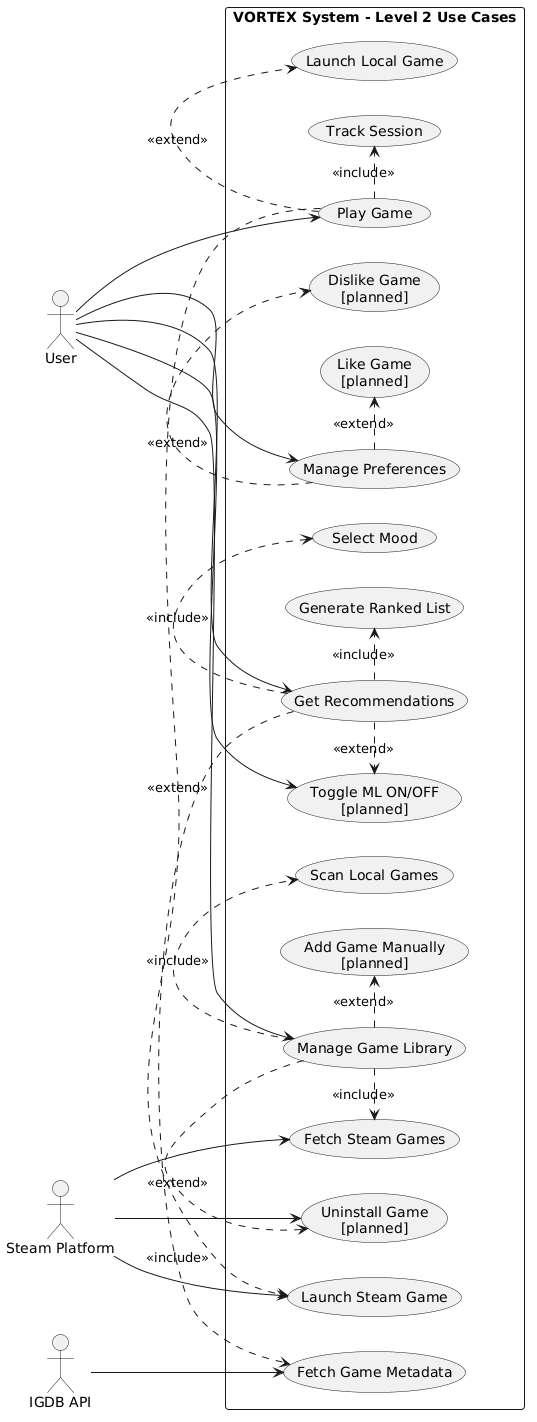
\includegraphics[height=1.5\textwidth]{../figures/level2 usecase diagram.png}
    \caption{Use Case Diagram Level-2 (Source: By Team)}
\end{figure}

\subsection{\underline{User Classes and Characteristics}}
\begin{itemize}
    \item \textbf{End User (Gamer)}
    \begin{itemize}
        \item Possesses basic technical knowledge.
        \item Requires a simple interaction model and low-latency system responses.
    \end{itemize}
    \item \textbf{Project Developer}
    \begin{itemize}
        \item Responsible for core modules (C++, Python, Database, and UI).
        \item Requires modular, decoupled, and testable components for iterative development.
    \end{itemize}
    \item \textbf{Evaluator / Faculty}
    \begin{itemize}
        \item Reviews the technical methodology, system architecture, and requirement traceability.
        \item Validates the alignment between project goals and final implementation.
    \end{itemize}
\end{itemize}



\subsection{\underline{Design and Implementation Constraints}}
\begin{itemize}
    \item \textbf{Primary OS Target}: System is specifically designed for the Windows operating system.
    \item \textbf{Steam Data Dependencies}: Retrieval relies on access to the Windows Registry and the local Steam file structure.
    \item \textbf{Local Discovery}: Local scanning logic currently assumes executable-based discovery targeting \texttt{.exe} files.
    \item \textbf{Recommendation Constraints}: Quality is contingent upon the completeness of metadata and the depth of available user history.
    \item \textbf{Temporal Constraints}: Project development is limited to a 12-week academic implementation window.
\end{itemize}

\newpage
\subsection{\underline{Design Diagrams}}
% \begin{figure}[H]
%     \centering
%     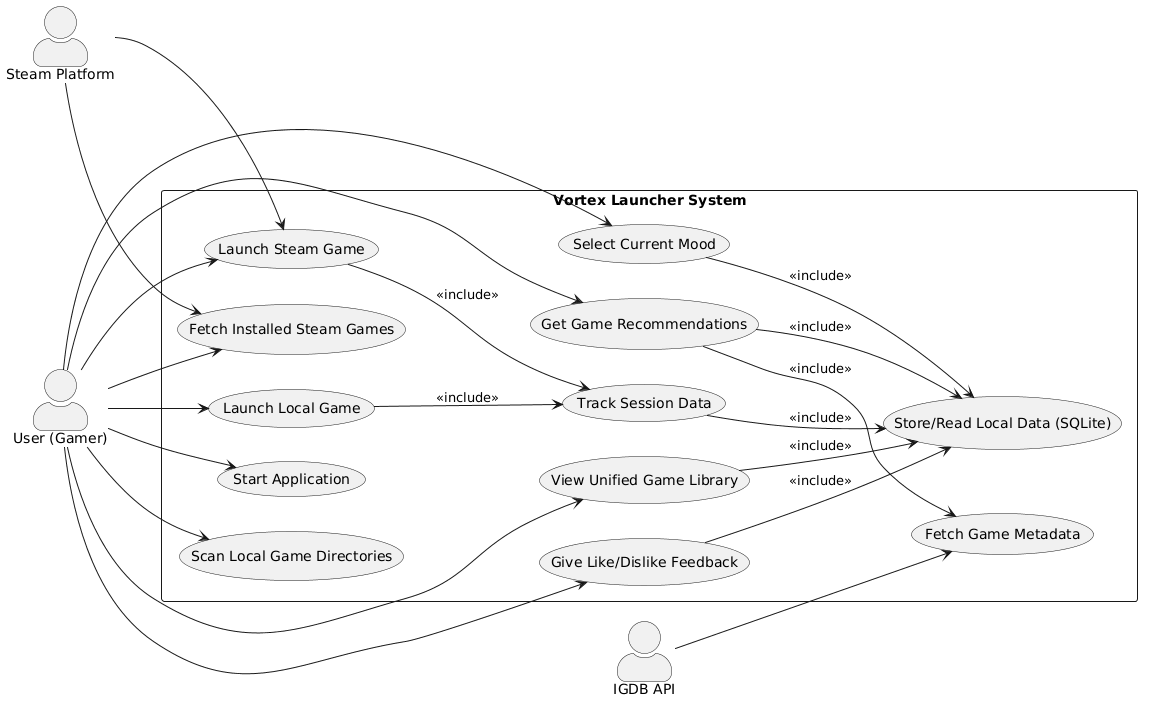
\includegraphics[width=0.75\textwidth,keepaspectratio]{../figures/usecase diagram.png}
%     \caption{Use Case Diagram}
% \end{figure}

\begin{figure}[H]
    \centering
    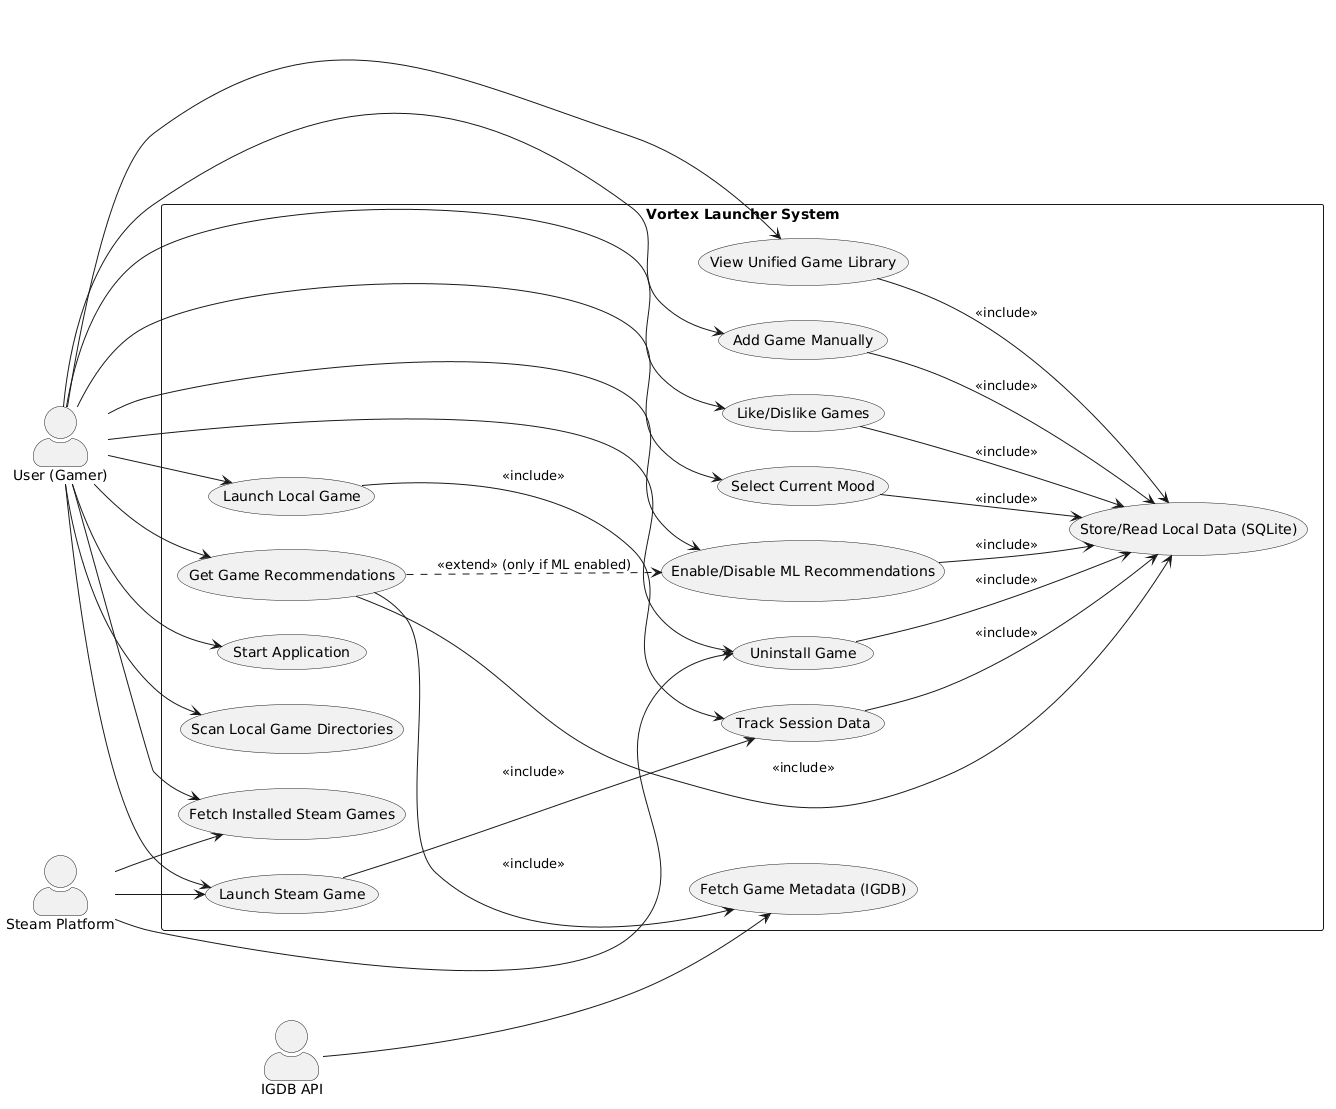
\includegraphics[angle=90, width=\textwidth, keepaspectratio]{../figures/usecase_diagram2.png}
    \caption{Use Case Diagram (Source: By Team)}
\end{figure}

\begin{figure}[H]
    \centering
    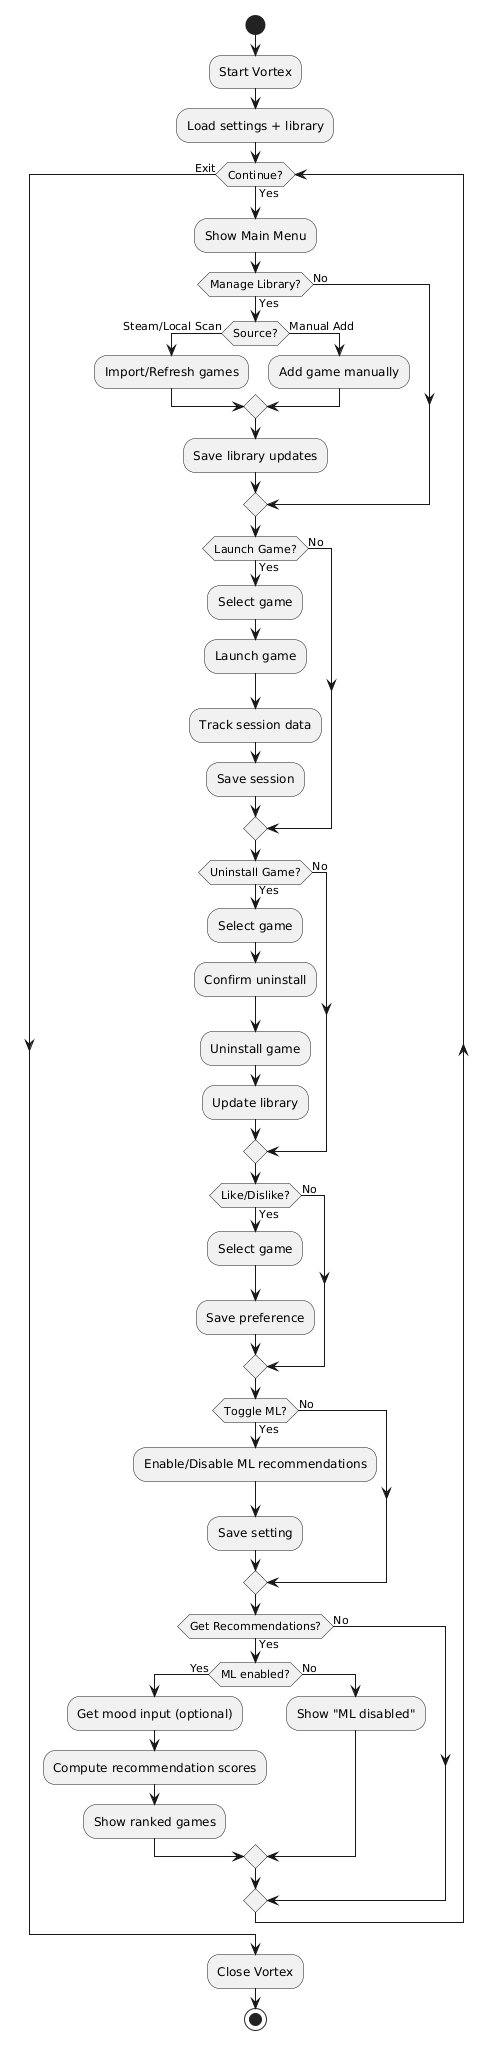
\includegraphics[height=\textheight,keepaspectratio]{../figures/ActivityDiagram_compact.png}
    \caption{Activity Diagram (Source: By Team)}
\end{figure}

% \begin{figure}[H]
%     \centering
%     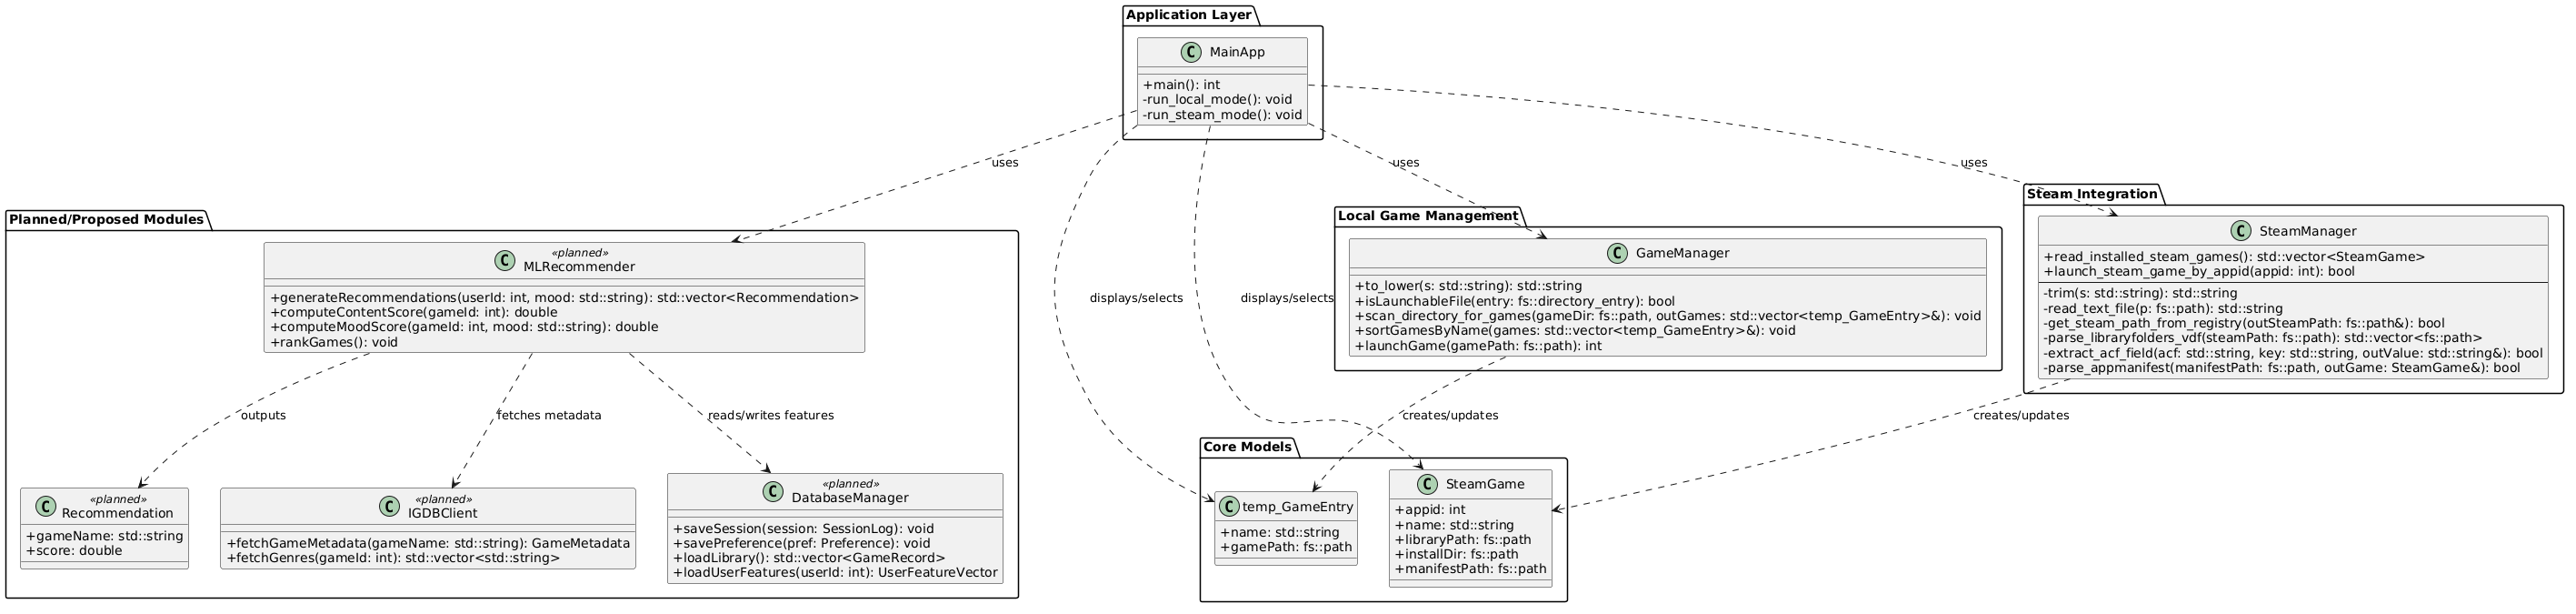
\includegraphics[width=0.9\textwidth]{../figures/class diagram.png}
%     \caption{Class Diagram}
% \end{figure}

\begin{figure}[H]
    \centering
    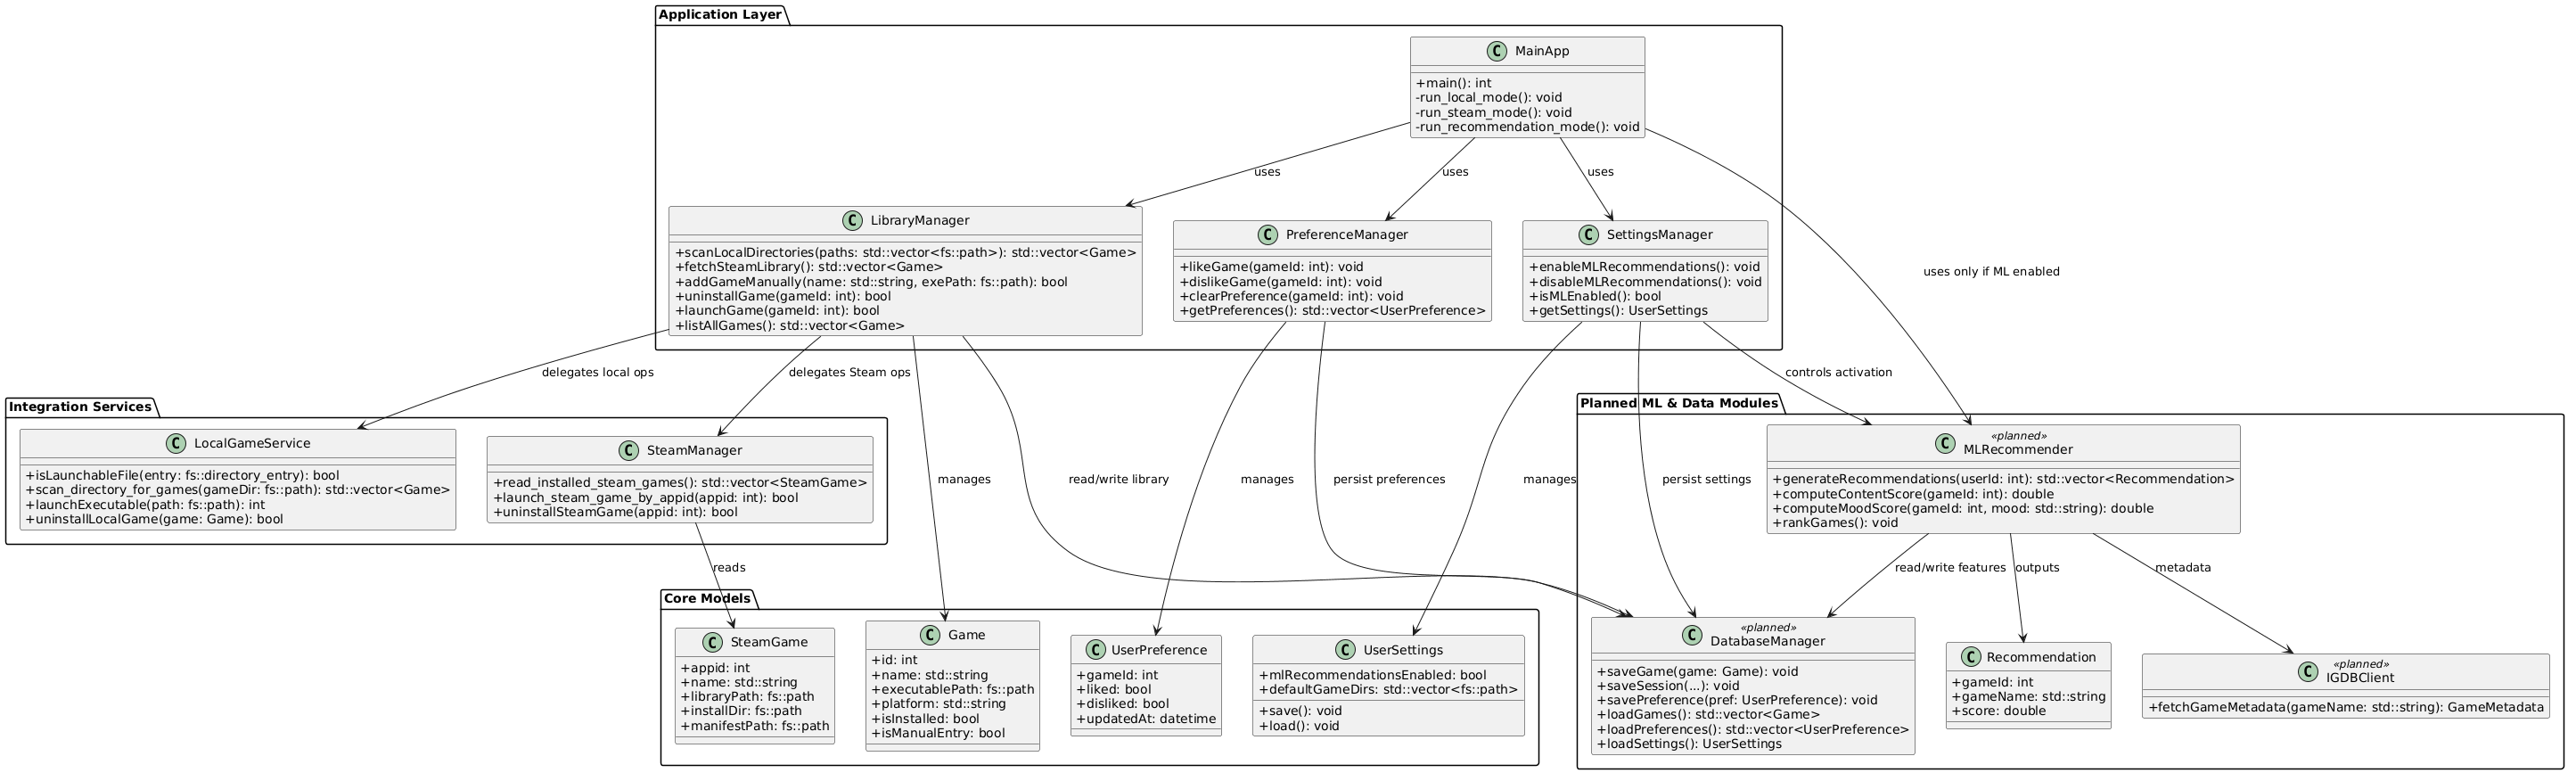
\includegraphics[angle=90, width=0.5\textwidth]{../figures/class_diagram2.png}
    \caption{Class Diagram 2 (Source: By Team)}
\end{figure}

\begin{figure}[H]
    \centering
    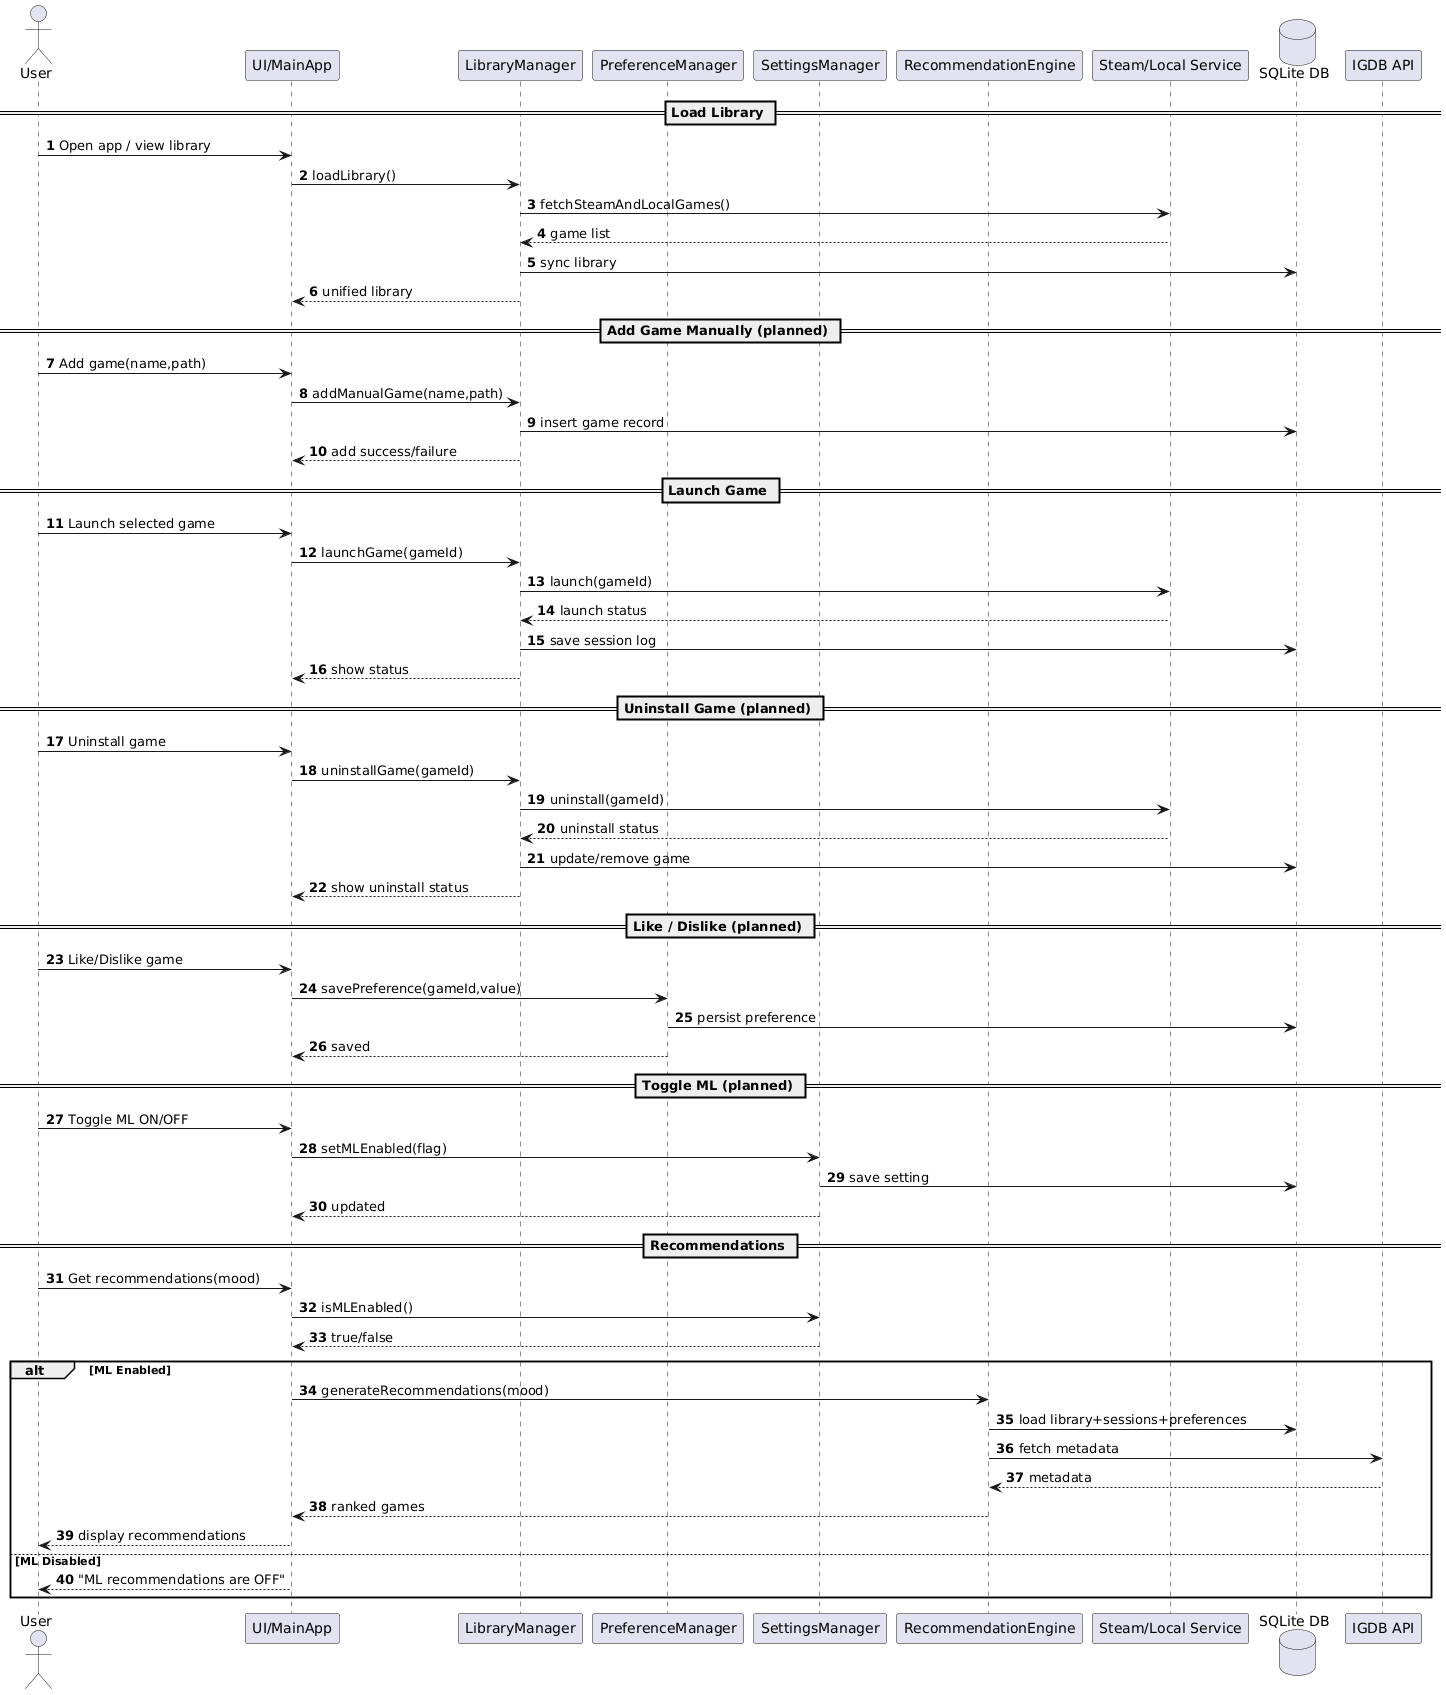
\includegraphics[width=\textwidth]{../figures/Sequence Diagram.png}
    \caption{Sequence Diagram (Source: By Team)}
\end{figure}

\begin{figure}[H]
    \centering
    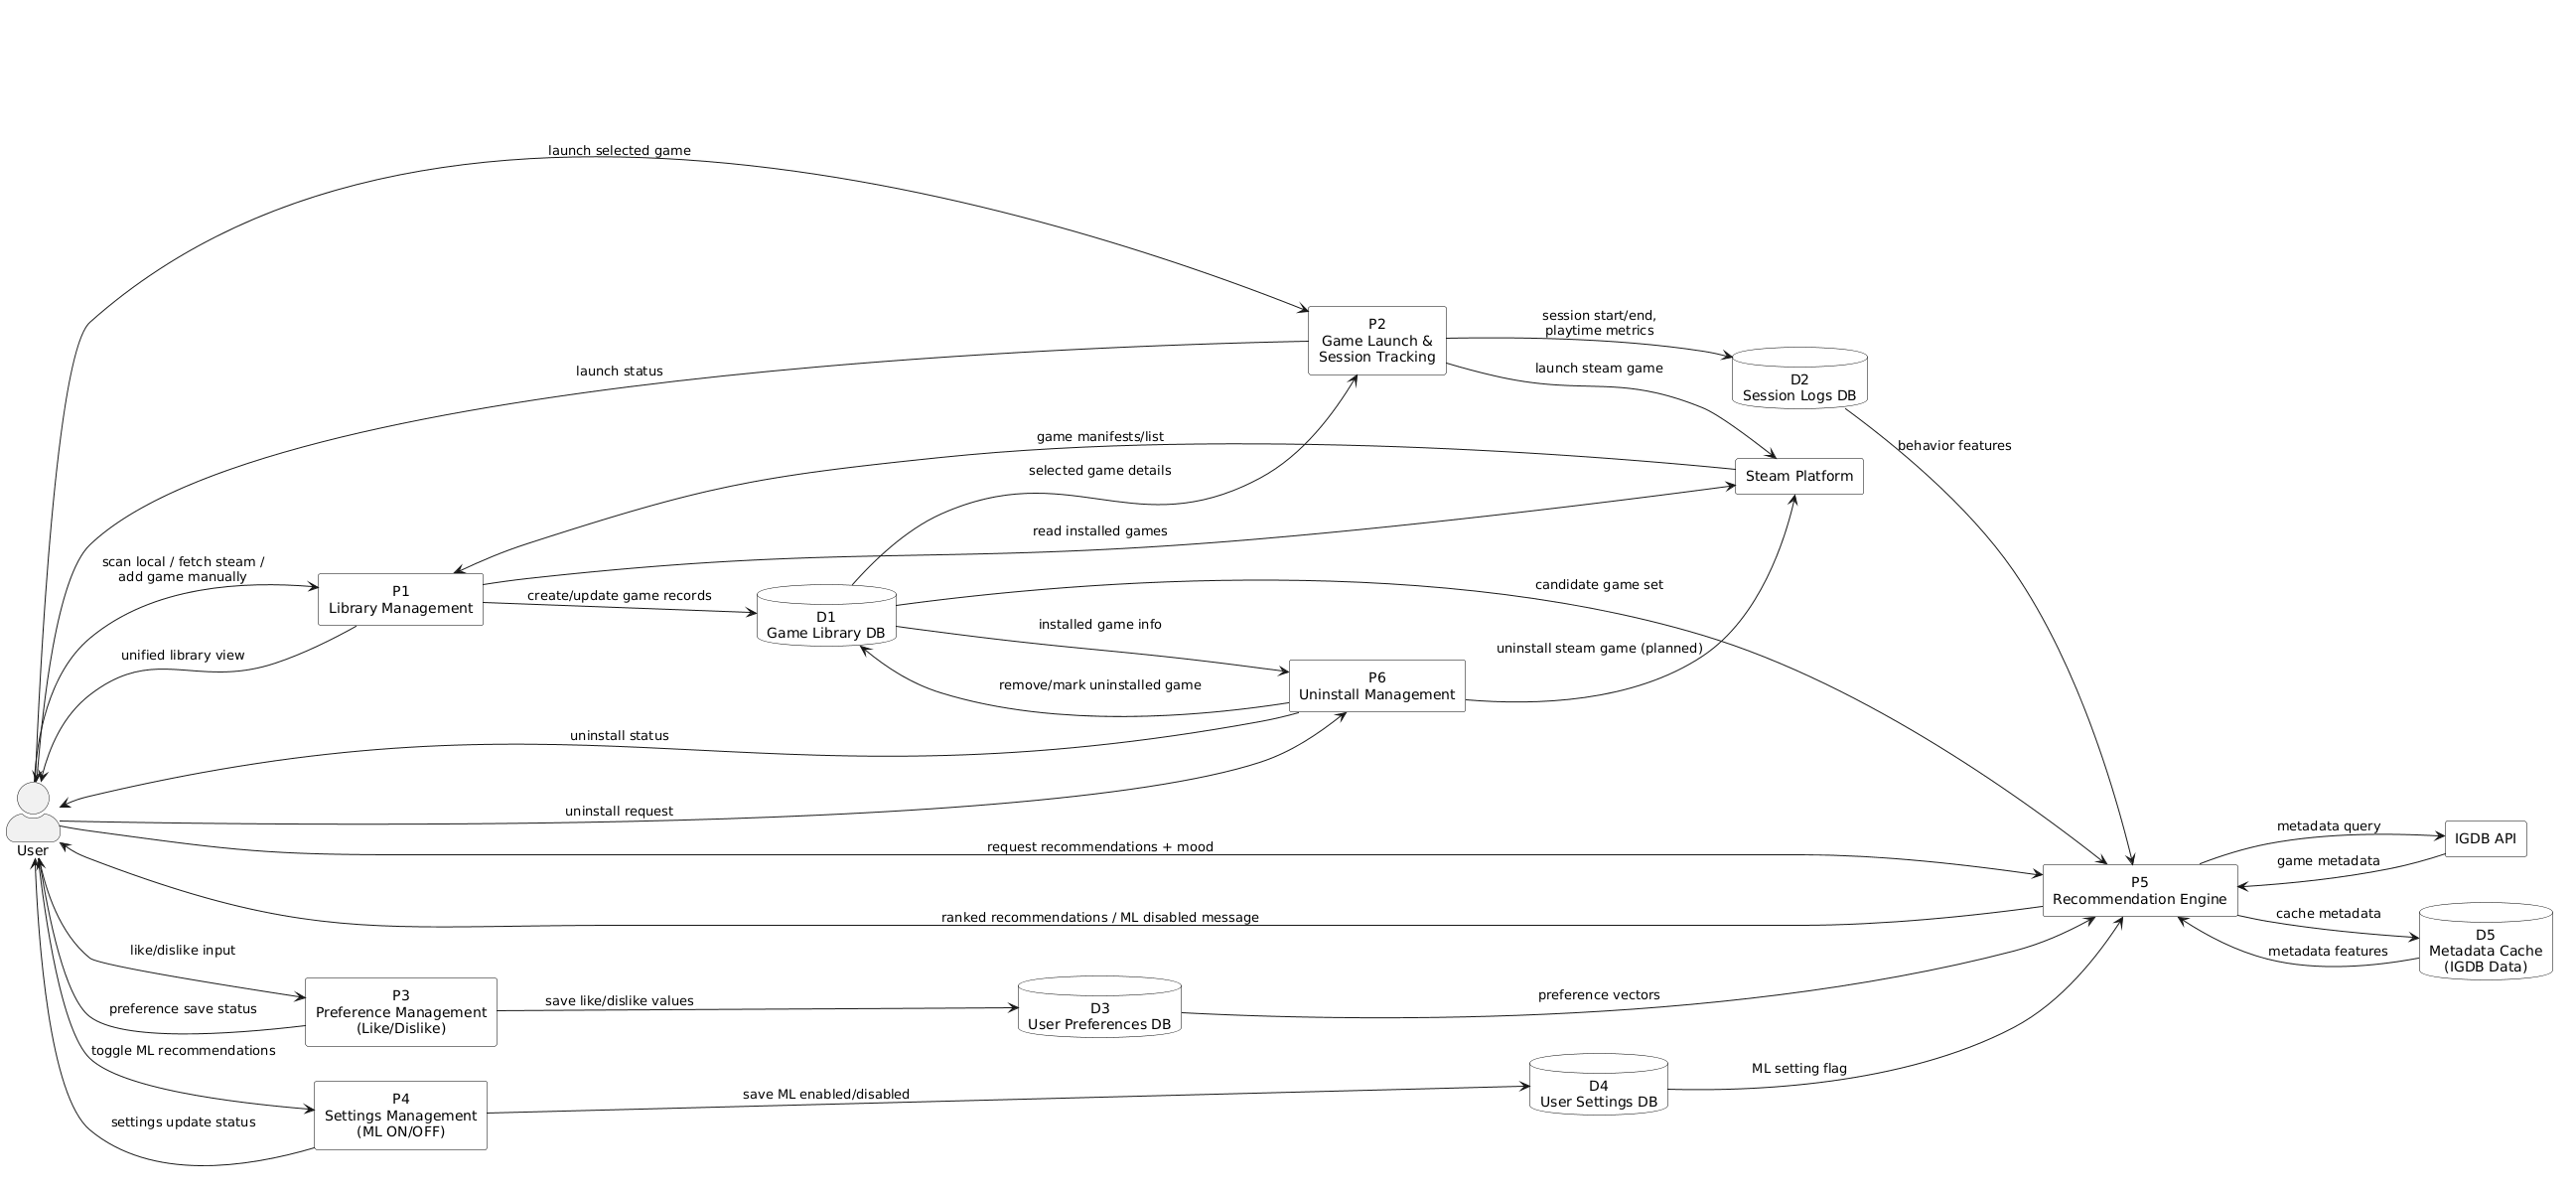
\includegraphics[angle=90, width=0.75\textwidth]{../figures/DFD.png}
    \caption{Data Flow Diagram (Source: By Team)}
\end{figure}

\begin{figure}[H]
    \centering
    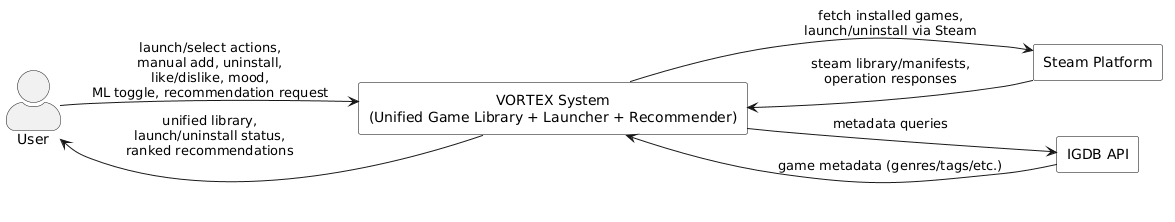
\includegraphics[angle=90, height=1.5\textwidth]{../figures/DFD level-0.png}
    \caption{Data Flow Diagram Level-0 (Source: By Team)}
\end{figure}

% \begin{figure}[H]
%     \centering
%     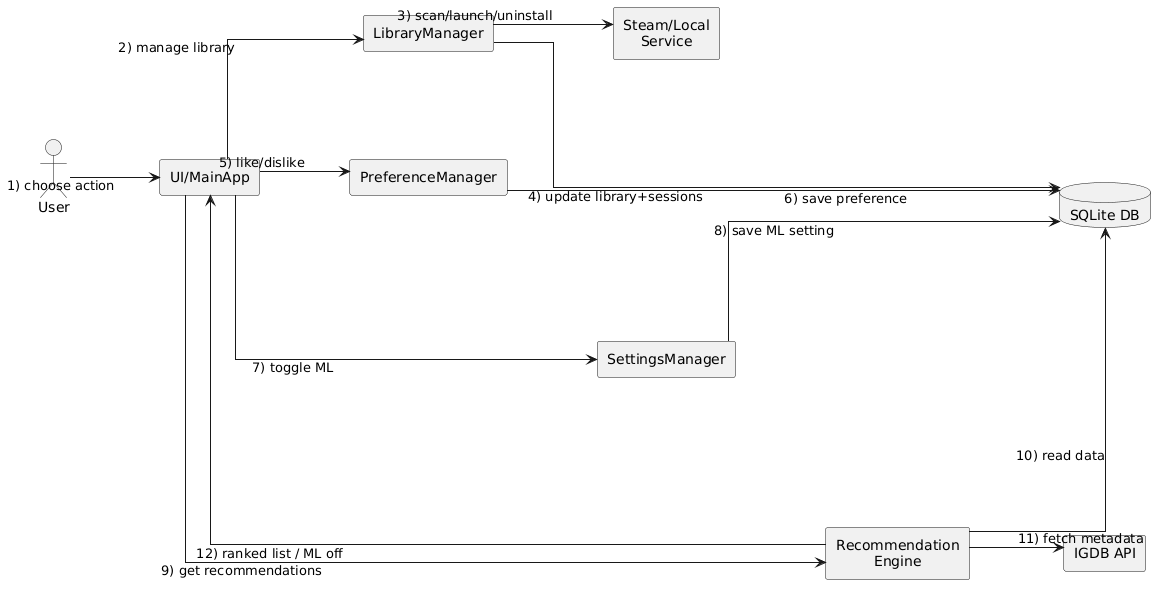
\includegraphics[width=0.8\textwidth]{../figures/Collaboration Diagram.png}
%     \caption{Collaboration Diagram}
% \end{figure}

\begin{figure}[H]
    \centering
    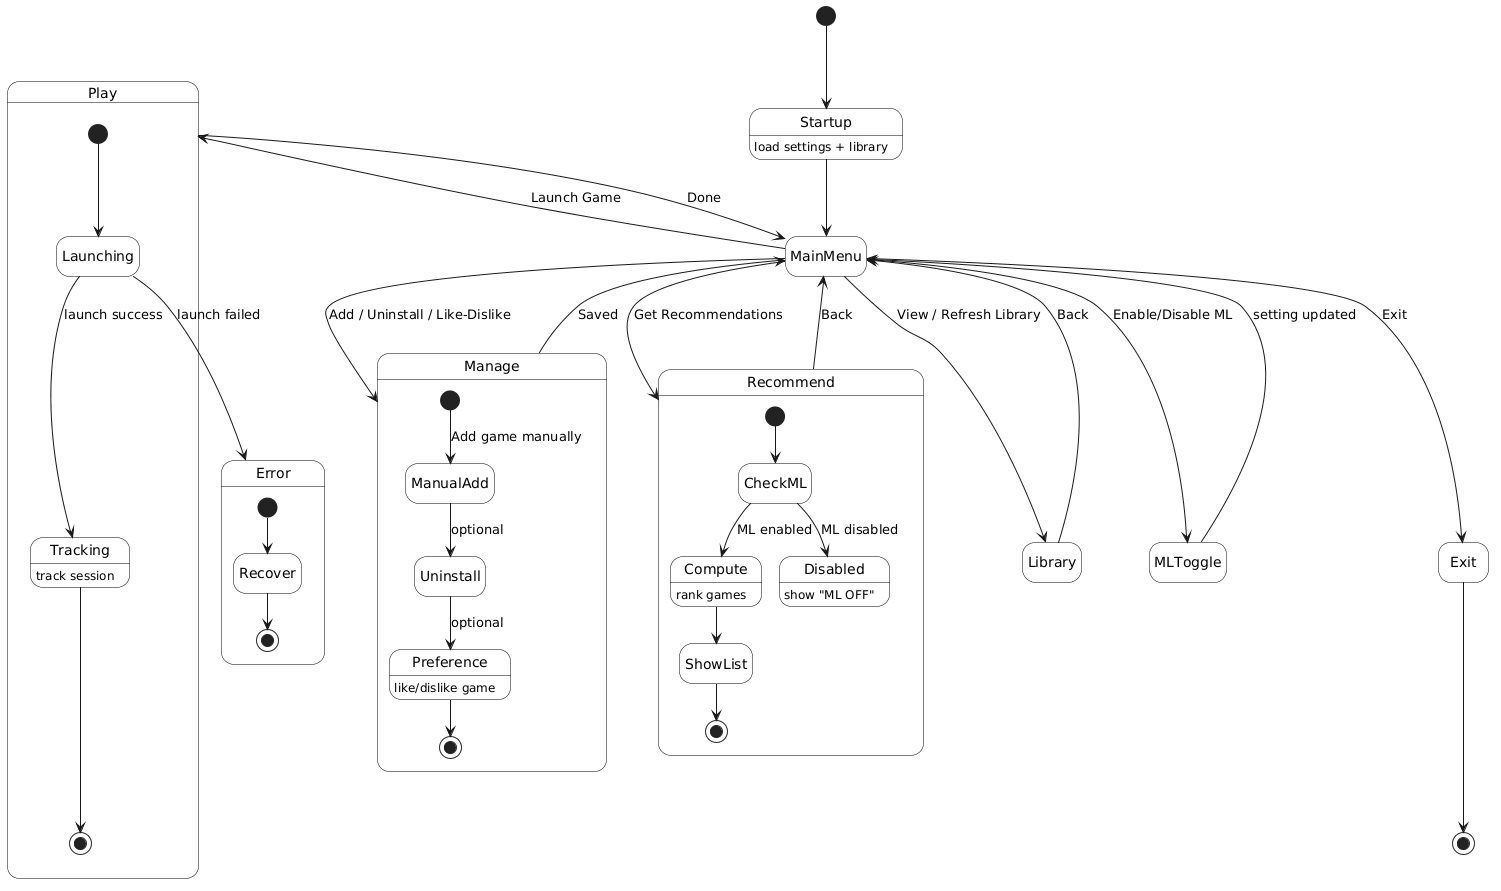
\includegraphics[angle=90, width=\textwidth]{../figures/State_diagram_compact.png}
    \caption{State Diagram (Source: By Team)}
\end{figure}

\subsection{\underline{Assumption and Dependencies}}
\begin{itemize}
    \item \textbf{Steam Installation}: The Steam client must be installed and accessible on the host machine.
    \item \textbf{Local Binaries}: User must have locally installed game binaries available for detection.
    \item \textbf{Network Connectivity}: Internet access is required for fetching external metadata via the IGDB API.
    \item \textbf{Environment Runtime}: Python runtime and all necessary machine learning libraries must be configured for the recommendation module.
    \item \textbf{System Permissions}: Appropriate administrative or user permissions are required for file system scanning and process initialization.
\end{itemize}

\section{SYSTEM REQUIREMENTS}

\subsection{\underline{User Interface}}
\begin{itemize}
    \item The current iteration of the user interface operates via a top-level Command Line Interface (CLI) menu, presenting options for Steam games, local directory games, and an exit function.
    \item The next iteration of the user interface is currently in development for a more modular and interactive experience.
    \item System shall display main menu with launcher modes.
    \item System shall display discovered games with index, title, and identifier/path.
    \item System shall allow user to select and launch game by input.
    \item System shall provide clear feedback for invalid input and launch failures.
    \item System shall display recommendation list with score in ranked order (when ML module invoked).
\end{itemize}

\subsection{\underline{Software Interface}}
\begin{itemize}

\item \textbf{C++ Core Modules}
    \begin{itemize}
	\item \texttt{game\_manager}: local directory scan, sorting, launch.
	\item \texttt{store\_manager}: Steam registry detection, library parsing, Steam launch.
    \end{itemize}

\item \textbf{Python Module}
    \begin{itemize}
	\item Metadata ingestion from IGDB.
	\item Feature extraction and score calculation.
    \end{itemize}

\item \textbf{Planned UI Layer}
    \begin{itemize}
	\item Qt/QML frontend over C++ backend services.
    \end{itemize}

\end{itemize}

\subsection{\underline{Database Interface}}
\begin{itemize}
    \item \textbf{Game catalog records}: Comprehensive data on available titles and assets.
    \item \textbf{Session logs}: Tracking metrics such as start time, end time, and total playtime.
    \item \textbf{User preference flags}: Binary or categorical data (e.g., like/dislike) for personalization.
    \item \textbf{Mood-session records}: Links between specific user moods and their corresponding gameplay sessions.
    \item \textbf{Cached metadata references}: Localized pointers to external assets for optimized performance.
\end{itemize}

\subsection{\underline{Protocols}}
\begin{itemize}
    \item \textbf{Local Process Execution}: Utilizing \texttt{ShellExecute} on Windows for native system calls.
    \item \textbf{Steam Launch Protocol}: Integration of the \texttt{steam://run/<appid>} URI for direct game initialization.
    \item \textbf{IGDB API Integration}: Secure HTTPS communication using Twitch OAuth for metadata retrieval.
    \item \textbf{Inter-Language Bridge}: Internal C++ $\leftrightarrow$ Python data exchange via file-based JSON or an API bridge.
\end{itemize}

\section{NON-FUNCTIONAL REQUIREMENTS}

\subsection{\underline{Performance Requirements}}
\begin{itemize}
    \item \textbf{Game List Retrieval}: Steam and local library fetching must complete within acceptable desktop latency for standard library sizes.
    \item \textbf{Resource Efficiency}: The launcher must avoid excessive memory usage during the scanning and ranking phases.
    \item \textbf{Interactive Performance}: Recommendation generation must complete within a user-tolerable timeframe for fluid usage.
\end{itemize}

\subsection{\underline{Security Requirements}}
\begin{itemize}
    \item \textbf{Secret Management}: No plaintext storage of external API secrets within the source code.
    \item \textbf{Input Validation}: All data from external files or APIs must be validated prior to processing.
    \item \textbf{Sandboxing}: File and process operations are strictly limited to intended game and application paths.
    \item \textbf{Data Privacy}: Local user data must remain on-device unless an explicit export is initiated.
\end{itemize}

\subsection{\underline{Software Quality Attributes}}
\begin{itemize}
    \item \textbf{Reliability}: Graceful handling of invalid paths, malformed manifests, and missing registry keys.
    \item \textbf{Maintainability}: Modular design featuring distinct components for \texttt{game\_manager}, \texttt{steam\_manager}, and the ML module.
    \item \textbf{Usability}: A simple, low-friction user flow to ensure an intuitive experience.
    \item \textbf{Portability}: A Windows-first architecture designed with future cross-platform compatibility in mind.
    \item \textbf{Scalability}: Support for expanding game libraries and additional data features over time.
\end{itemize}

\section{OTHER REQUIREMENTS}
\subsection{\underline{Evaluation-Oriented Requirements}}
    \begin{itemize}
        \item Include requirement traceability mapping (Requirement $\rightarrow$ Module $\rightarrow$ Test Case).
        \item Provide evidence screenshots and logs for scanning, launching, and recommendation output.
    \end{itemize}

\subsection{\underline{Testing Requirements}}
    \begin{itemize}
        \item \textbf{Unit Tests}: Coverage for parsing and scanning logic.
        \item \textbf{Integration Tests}: Verification of Steam detection and the end-to-end launch flow.
        \item \textbf{Validation Tests}: Evaluation of recommendation quality using precision@k and sanity checks.
    \end{itemize}

    \subsection{\underline{Documentation Requirements}}
    \begin{itemize}
        \item \textbf{User Manual}: Comprehensive instructions for installation and usage.
        \item \textbf{Developer Setup Guide}: Detailed steps for build processes, dependencies, and execution.
        \item \textbf{Project Roadmap}: Documentation of known limitations and planned future work.
    \end{itemize}


\appendix

\clearpage
\section{Glossary}

\begin{description}

\item[IGDB]
Internet Game Database; a large structured database of video game information used to programmatically fetch game metadata via its official API.

\item[Launcher]
An interface or application that opens a game executable upon user input.

\item[One-Hot Encoding]
A machine learning technique used to convert categorical data (such as user moods or game genres) into a numerical binary format.

\item[Platforms]
Digital game distribution services (e.g., Steam, GOG, Epic Games Store) where users purchase, subscribe to, and manage games.

\item[TF--IDF Vectorizer]
Term Frequency – Inverse Document Frequency; a technique used to convert text documents (such as game descriptions) into numerical vectors that machine learning models can process.

\end{description}

\section{Analysis Model}

\begin{description}

\item[Data to ML Quantification Pipeline]
The primary analysis model used to process raw system data into machine-readable formats. 
This pipeline converts text descriptions into TF--IDF float vectors, playtime into normalized
values scaled between 0 and 1, and time-of-day information into temporal encodings.

\item[Engagement Score Calculation Model]
An analytical model that computes user engagement with a game by calculating a weighted
combination of the following components:

\begin{itemize}
\item Playtime Score
\item Frequency Score
\item Length Score
\end{itemize}

\item[Hybrid Ranker Model]
The final analysis model responsible for generating recommendations. It calculates a final
recommendation score between 0.0 and 1.0 using the following weighted components:

\begin{itemize}
\item Preference Match (0.40)
\item Similarity to Liked Games (0.35)
\item Quality Score (0.15)
\item Exploration Factor (0.10)
\end{itemize}

\end{description}

\section{Issues List}

\subsection*{Open Issues}

\begin{itemize}

\item The machine learning recommendation module currently yields inconsistent recommendation
quality. The Python implementation remains a work in progress and requires further calibration.

\item The intended Qt/QML user interface design is not yet finalized.

\item The system experiences the \textit{Cold Start} data sparsity problem for new users with zero
recorded playtime. This is currently mitigated by asking users to manually select preferred
genres during the initial setup process.

\end{itemize}

\subsection*{Resolved Issues}

\begin{itemize}

\item The project environment previously failed to place \texttt{std::filesystem} in a namespace.
This issue was resolved by upgrading the project standard from C++14 to C++17.

\item The local heuristic game scanner initially detected redundant executables such as crash
handlers and uninstallers. This issue was resolved by implementing block parameters for
undesired executable names and applying a heuristic that selects the largest executable file.

\end{itemize}


% \printbibliography

\end{document}
